% Options for packages loaded elsewhere
\PassOptionsToPackage{unicode}{hyperref}
\PassOptionsToPackage{hyphens}{url}
\PassOptionsToPackage{dvipsnames,svgnames,x11names}{xcolor}
%
\documentclass[
]{article}
\usepackage{amsmath,amssymb}
\usepackage{iftex}
\ifPDFTeX
  \usepackage[T1]{fontenc}
  \usepackage[utf8]{inputenc}
  \usepackage{textcomp} % provide euro and other symbols
\else % if luatex or xetex
  \usepackage{unicode-math} % this also loads fontspec
  \defaultfontfeatures{Scale=MatchLowercase}
  \defaultfontfeatures[\rmfamily]{Ligatures=TeX,Scale=1}
\fi
\usepackage{lmodern}
\ifPDFTeX\else
  % xetex/luatex font selection
\fi
% Use upquote if available, for straight quotes in verbatim environments
\IfFileExists{upquote.sty}{\usepackage{upquote}}{}
\IfFileExists{microtype.sty}{% use microtype if available
  \usepackage[]{microtype}
  \UseMicrotypeSet[protrusion]{basicmath} % disable protrusion for tt fonts
}{}
\makeatletter
\@ifundefined{KOMAClassName}{% if non-KOMA class
  \IfFileExists{parskip.sty}{%
    \usepackage{parskip}
  }{% else
    \setlength{\parindent}{0pt}
    \setlength{\parskip}{6pt plus 2pt minus 1pt}}
}{% if KOMA class
  \KOMAoptions{parskip=half}}
\makeatother
\usepackage{xcolor}
\usepackage[margin=1in]{geometry}
\usepackage{color}
\usepackage{fancyvrb}
\newcommand{\VerbBar}{|}
\newcommand{\VERB}{\Verb[commandchars=\\\{\}]}
\DefineVerbatimEnvironment{Highlighting}{Verbatim}{commandchars=\\\{\}}
% Add ',fontsize=\small' for more characters per line
\usepackage{framed}
\definecolor{shadecolor}{RGB}{248,248,248}
\newenvironment{Shaded}{\begin{snugshade}}{\end{snugshade}}
\newcommand{\AlertTok}[1]{\textcolor[rgb]{0.94,0.16,0.16}{#1}}
\newcommand{\AnnotationTok}[1]{\textcolor[rgb]{0.56,0.35,0.01}{\textbf{\textit{#1}}}}
\newcommand{\AttributeTok}[1]{\textcolor[rgb]{0.13,0.29,0.53}{#1}}
\newcommand{\BaseNTok}[1]{\textcolor[rgb]{0.00,0.00,0.81}{#1}}
\newcommand{\BuiltInTok}[1]{#1}
\newcommand{\CharTok}[1]{\textcolor[rgb]{0.31,0.60,0.02}{#1}}
\newcommand{\CommentTok}[1]{\textcolor[rgb]{0.56,0.35,0.01}{\textit{#1}}}
\newcommand{\CommentVarTok}[1]{\textcolor[rgb]{0.56,0.35,0.01}{\textbf{\textit{#1}}}}
\newcommand{\ConstantTok}[1]{\textcolor[rgb]{0.56,0.35,0.01}{#1}}
\newcommand{\ControlFlowTok}[1]{\textcolor[rgb]{0.13,0.29,0.53}{\textbf{#1}}}
\newcommand{\DataTypeTok}[1]{\textcolor[rgb]{0.13,0.29,0.53}{#1}}
\newcommand{\DecValTok}[1]{\textcolor[rgb]{0.00,0.00,0.81}{#1}}
\newcommand{\DocumentationTok}[1]{\textcolor[rgb]{0.56,0.35,0.01}{\textbf{\textit{#1}}}}
\newcommand{\ErrorTok}[1]{\textcolor[rgb]{0.64,0.00,0.00}{\textbf{#1}}}
\newcommand{\ExtensionTok}[1]{#1}
\newcommand{\FloatTok}[1]{\textcolor[rgb]{0.00,0.00,0.81}{#1}}
\newcommand{\FunctionTok}[1]{\textcolor[rgb]{0.13,0.29,0.53}{\textbf{#1}}}
\newcommand{\ImportTok}[1]{#1}
\newcommand{\InformationTok}[1]{\textcolor[rgb]{0.56,0.35,0.01}{\textbf{\textit{#1}}}}
\newcommand{\KeywordTok}[1]{\textcolor[rgb]{0.13,0.29,0.53}{\textbf{#1}}}
\newcommand{\NormalTok}[1]{#1}
\newcommand{\OperatorTok}[1]{\textcolor[rgb]{0.81,0.36,0.00}{\textbf{#1}}}
\newcommand{\OtherTok}[1]{\textcolor[rgb]{0.56,0.35,0.01}{#1}}
\newcommand{\PreprocessorTok}[1]{\textcolor[rgb]{0.56,0.35,0.01}{\textit{#1}}}
\newcommand{\RegionMarkerTok}[1]{#1}
\newcommand{\SpecialCharTok}[1]{\textcolor[rgb]{0.81,0.36,0.00}{\textbf{#1}}}
\newcommand{\SpecialStringTok}[1]{\textcolor[rgb]{0.31,0.60,0.02}{#1}}
\newcommand{\StringTok}[1]{\textcolor[rgb]{0.31,0.60,0.02}{#1}}
\newcommand{\VariableTok}[1]{\textcolor[rgb]{0.00,0.00,0.00}{#1}}
\newcommand{\VerbatimStringTok}[1]{\textcolor[rgb]{0.31,0.60,0.02}{#1}}
\newcommand{\WarningTok}[1]{\textcolor[rgb]{0.56,0.35,0.01}{\textbf{\textit{#1}}}}
\usepackage{graphicx}
\makeatletter
\def\maxwidth{\ifdim\Gin@nat@width>\linewidth\linewidth\else\Gin@nat@width\fi}
\def\maxheight{\ifdim\Gin@nat@height>\textheight\textheight\else\Gin@nat@height\fi}
\makeatother
% Scale images if necessary, so that they will not overflow the page
% margins by default, and it is still possible to overwrite the defaults
% using explicit options in \includegraphics[width, height, ...]{}
\setkeys{Gin}{width=\maxwidth,height=\maxheight,keepaspectratio}
% Set default figure placement to htbp
\makeatletter
\def\fps@figure{htbp}
\makeatother
\setlength{\emergencystretch}{3em} % prevent overfull lines
\providecommand{\tightlist}{%
  \setlength{\itemsep}{0pt}\setlength{\parskip}{0pt}}
\setcounter{secnumdepth}{-\maxdimen} % remove section numbering
\usepackage{color}
\ifLuaTeX
  \usepackage{selnolig}  % disable illegal ligatures
\fi
\IfFileExists{bookmark.sty}{\usepackage{bookmark}}{\usepackage{hyperref}}
\IfFileExists{xurl.sty}{\usepackage{xurl}}{} % add URL line breaks if available
\urlstyle{same}
\hypersetup{
  pdftitle={Assigment 2},
  pdfauthor={Luis Hinostroza},
  colorlinks=true,
  linkcolor={Maroon},
  filecolor={Maroon},
  citecolor={Blue},
  urlcolor={blue},
  pdfcreator={LaTeX via pandoc}}

\title{Assigment 2}
\author{Luis Hinostroza}
\date{2023-10-06}

\begin{document}
\maketitle

\hypertarget{questions-about-cars-from-the-auto-dataset.}{%
\subsection{Questions about Cars from the ``Auto''
Dataset.}\label{questions-about-cars-from-the-auto-dataset.}}

In this study we used a dataset ``Auto'' of different cars between
1970's and 1980's from three origins: America (1), European (2), and
Japanese (3).

I found that there is a close relationship between all variables. Every
variable depend from each other and their values are numerical and
categorical. Also, a good source for understanding how and why the mpg,
weight, cylinder, horsepower, and displacement can affect the
consumption of gas, the time in acceleration, and the size of the
engine.

We use different plots like scatterplot, boxplot, mosaic plot, and bar
plot. We also use the correlation, chi-squared test, and anova test to
understand relationship and if there are statistically significant
difference.

Overall, this study is to understand and visualize the data in a more
friendly and easy representation of it.

\newpage

\hypertarget{q01---does-more-horsepower-decreases-the-acceleration-time}{%
\subsection{Q\#01 - Does more horsepower decreases the acceleration
time?}\label{q01---does-more-horsepower-decreases-the-acceleration-time}}

Looking at the graph we can notice there is a relation between hp and
acceleration. The more hp the less time accelerating. Also the
correlation coefficient represent a pretty strong linear relation.

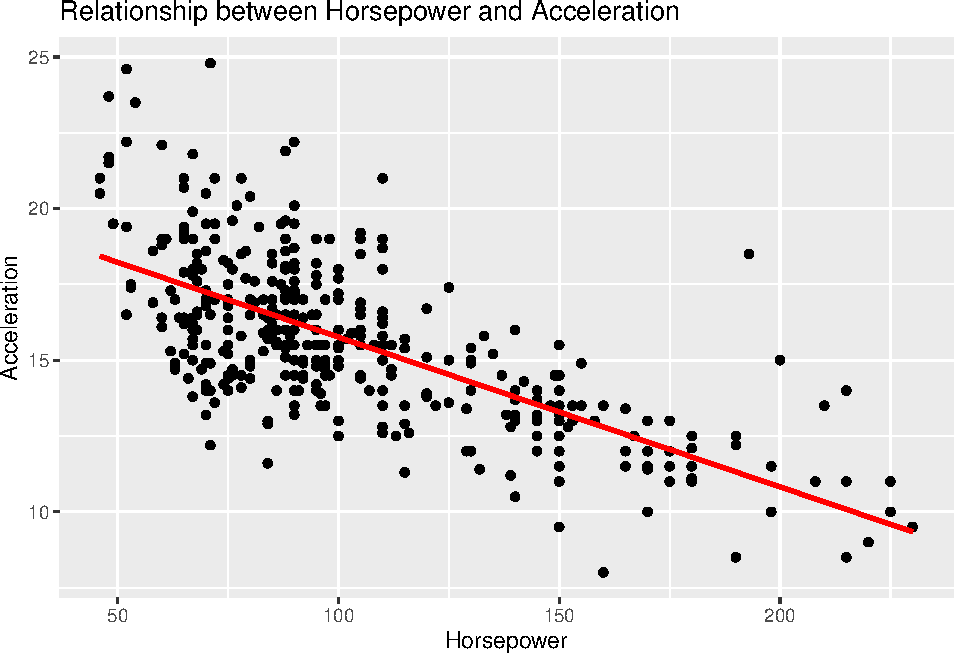
\includegraphics{QuestionCar_files/figure-latex/unnamed-chunk-1-1.pdf}

\begin{verbatim}
## [1] -0.6891955
\end{verbatim}

\newpage

\hypertarget{q02---does-the-mpg-depends-on-the-amount-of-cylinders}{%
\subsection{Q\#02 - Does the mpg depends on the amount of
cylinders?}\label{q02---does-the-mpg-depends-on-the-amount-of-cylinders}}

The graph shows that the right amount of cylinder can improve the mpg,
Four cylinders been the most efficient miles per gallons. The p-value
from the ANOVA test shows there's a statistically significant difference
in the mean mpg across different cylinders groups.

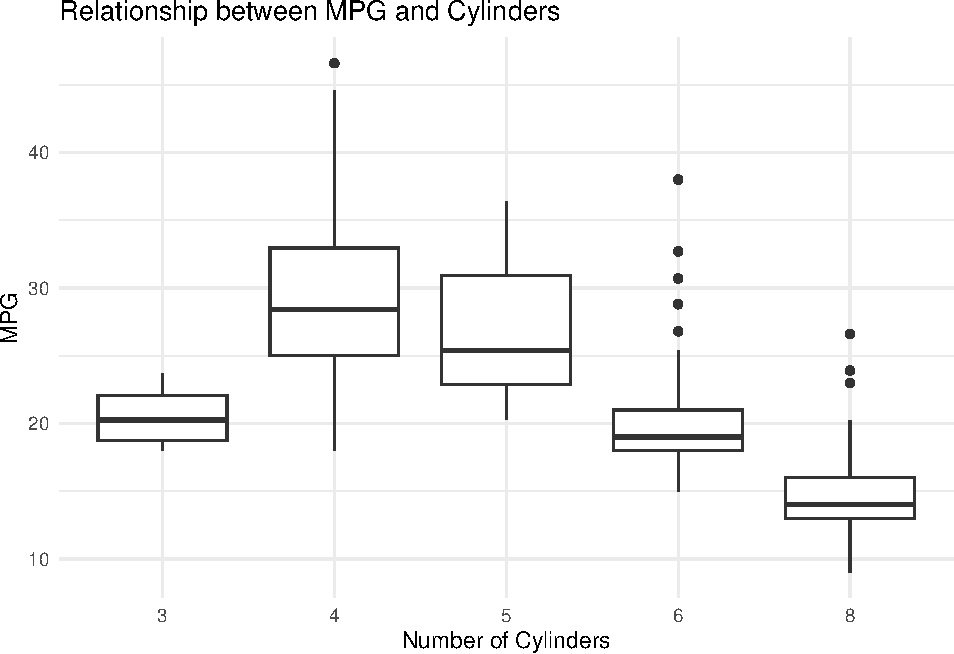
\includegraphics{QuestionCar_files/figure-latex/unnamed-chunk-2-1.pdf}

\begin{verbatim}
##                       Df Sum Sq Mean Sq F value Pr(>F)    
## as.factor(cylinders)   4  15275    3819     173 <2e-16 ***
## Residuals            387   8544      22                   
## ---
## Signif. codes:  0 '***' 0.001 '**' 0.01 '*' 0.05 '.' 0.1 ' ' 1
\end{verbatim}

\newpage

\hypertarget{q03---is-the-amount-of-cylinders-related-to-the-origin}{%
\subsection{Q\#03 - Is the amount of cylinders related to the
origin?}\label{q03---is-the-amount-of-cylinders-related-to-the-origin}}

We can notice from the graph the distribution of car by number of
cylinders. Orange being American (1), pink European (2), and red
Japanese (3). The p-value indicates that the two variables are not
independent and that there is a significant association between
cylinders and origin.

\begin{verbatim}
##    
##       1   2   3
##   3   0   0   4
##   4  69  61  69
##   5   0   3   0
##   6  73   4   6
##   8 103   0   0
\end{verbatim}

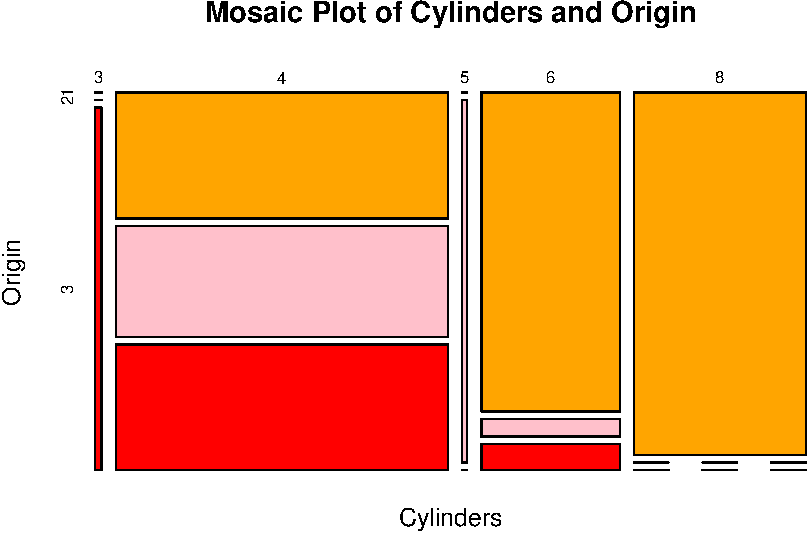
\includegraphics{QuestionCar_files/figure-latex/unnamed-chunk-3-1.pdf}

\begin{verbatim}
## 
##  Pearson's Chi-squared test
## 
## data:  table_cyl_origin
## X-squared = 180.72, df = 8, p-value < 2.2e-16
\end{verbatim}

\newpage

\hypertarget{q04---is-there-a-relation-between-the-displacement-and-weight}{%
\subsection{Q\#04 - Is there a relation between the displacement and
weight?}\label{q04---is-there-a-relation-between-the-displacement-and-weight}}

We can see on the plot that the points follow the red line affirming the
linear relation between both variables, proving that weight is related
to it displacement. And, the correlation coefficient indicates a strong
linear relationship as well.

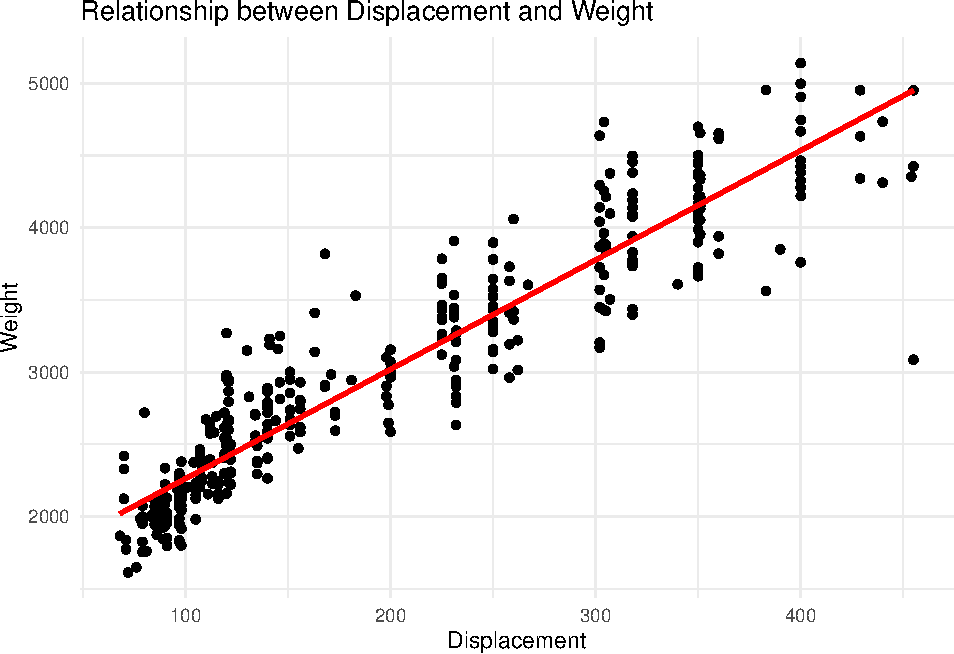
\includegraphics{QuestionCar_files/figure-latex/unnamed-chunk-4-1.pdf}

\begin{verbatim}
## [1] 0.9329944
\end{verbatim}

\newpage

\hypertarget{q05---what-is-the-percentage-of-cars-by-origin}{%
\subsection{Q\#05 - What is the percentage of cars by
origin?}\label{q05---what-is-the-percentage-of-cars-by-origin}}

It would be interesting to observe the amount and percentage of cars by
origin. The chart shows that mostly all cars come from America (1),
following by Japan (3).

Amount of cars by origin.

\begin{verbatim}
## 
##   1   2   3 
## 245  68  79
\end{verbatim}

Percentage of cars by origin.

\begin{verbatim}
## 
##        1        2        3 
## 62.50000 17.34694 20.15306
\end{verbatim}

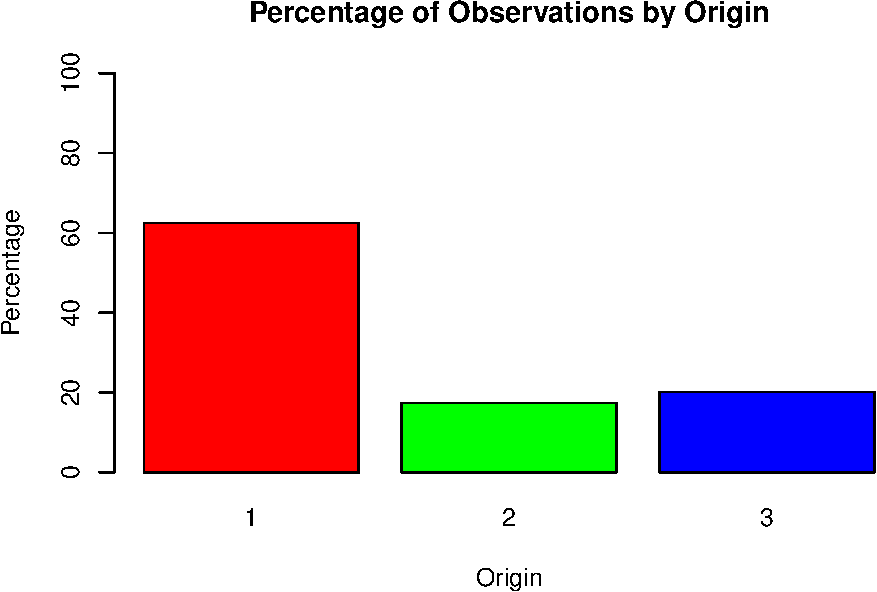
\includegraphics{QuestionCar_files/figure-latex/unnamed-chunk-6-1.pdf}

\newpage

\hypertarget{limitations-of-report}{%
\subsection{Limitations of Report:}\label{limitations-of-report}}

\begin{itemize}
\item
  The dataset contains a limited set of variables, which may not capture
  all factors influencing car characteristics and performance. For
  comprehensive analysis, we may need more variables or features.
\item
  The origin variable is represented as numerical values (1 for
  American, 2 for European, and 3 for Japanese). This is very misleading
  as they are categorical values.
\item
  The dataset is relatively old, as it shows cara from the 70s and 80s.
  The relationships and trends observed in this dataset may not be
  representative of modern cars due to new technologies, changes in
  manufacturing practices, and shifts in consumer preferences.
\item
  While the dataset provides various attributes for cars, it might lack
  other definitions or details for each variable, which can lead to
  misinterpretation or misuse of the data.
\end{itemize}

\newpage

\begin{itemize}
\tightlist
\item
  For question \#1: We visualize the relationship of the data between
  horsepower and Acceleration with a scatterplot and a linear fit. We
  also found the correlation coefficient.
\end{itemize}

\begin{Shaded}
\begin{Highlighting}[]
\FunctionTok{library}\NormalTok{(ggplot2)}
\FunctionTok{library}\NormalTok{(ISLR)}
\FunctionTok{library}\NormalTok{(dplyr)}
\NormalTok{hp\_acce }\OtherTok{\textless{}{-}} \FunctionTok{select}\NormalTok{(Auto, horsepower, acceleration)}
\FunctionTok{ggplot}\NormalTok{(hp\_acce, }\FunctionTok{aes}\NormalTok{(}\AttributeTok{x =}\NormalTok{ horsepower, }\AttributeTok{y =}\NormalTok{ acceleration)) }\SpecialCharTok{+}
  \FunctionTok{geom\_point}\NormalTok{() }\SpecialCharTok{+}
  \FunctionTok{geom\_smooth}\NormalTok{(}\AttributeTok{method =} \StringTok{"lm"}\NormalTok{, }\AttributeTok{se =} \ConstantTok{FALSE}\NormalTok{, }\AttributeTok{color =} \StringTok{"red"}\NormalTok{) }\SpecialCharTok{+}
  \FunctionTok{labs}\NormalTok{(}\AttributeTok{title =} \StringTok{"Relationship between Horsepower and Acceleration"}\NormalTok{,}
       \AttributeTok{x =} \StringTok{"Horsepower"}\NormalTok{,}
       \AttributeTok{y =} \StringTok{"Acceleration"}\NormalTok{)}
\FunctionTok{cor}\NormalTok{(Auto}\SpecialCharTok{$}\NormalTok{horsepower, Auto}\SpecialCharTok{$}\NormalTok{acceleration)}
\end{Highlighting}
\end{Shaded}

\begin{itemize}
\tightlist
\item
  For question \#2: We visualize the relationship of the data between
  mpg and cylinders with a boxplot. Each box represents the
  interquartile range of mpg for a specific number of cylinders. We also
  found the p-value from the ANOVA test to find out if there's a
  statistically significant difference in the mean mpg across different
  cylinders
\end{itemize}

\begin{Shaded}
\begin{Highlighting}[]
\FunctionTok{library}\NormalTok{(ggplot2)}
\FunctionTok{library}\NormalTok{(ISLR)}
\FunctionTok{library}\NormalTok{(dplyr)}
\NormalTok{mpg\_cyl }\OtherTok{\textless{}{-}} \FunctionTok{select}\NormalTok{(Auto, mpg, cylinders)}
\FunctionTok{ggplot}\NormalTok{(mpg\_cyl, }\FunctionTok{aes}\NormalTok{(}\AttributeTok{x =} \FunctionTok{as.factor}\NormalTok{(cylinders), }\AttributeTok{y =}\NormalTok{ mpg)) }\SpecialCharTok{+}
  \FunctionTok{geom\_boxplot}\NormalTok{() }\SpecialCharTok{+}
  \FunctionTok{labs}\NormalTok{(}\AttributeTok{title =} \StringTok{"Relationship between MPG and Cylinders"}\NormalTok{,}
       \AttributeTok{x =} \StringTok{"Number of Cylinders"}\NormalTok{,}
       \AttributeTok{y =} \StringTok{"MPG"}\NormalTok{) }\SpecialCharTok{+}
  \FunctionTok{theme\_minimal}\NormalTok{()}

\NormalTok{anova\_result }\OtherTok{\textless{}{-}} \FunctionTok{aov}\NormalTok{(mpg }\SpecialCharTok{\textasciitilde{}} \FunctionTok{as.factor}\NormalTok{(cylinders), }\AttributeTok{data =}\NormalTok{ Auto)}
\FunctionTok{summary}\NormalTok{(anova\_result)}
\end{Highlighting}
\end{Shaded}

\begin{itemize}
\tightlist
\item
  For question \#3: We created a contingency table to show the frequency
  distribution of the variables ina matrix format. We also created a
  mosaic plot to visualize the proportion to the number of cases in each
  category. We also found the chi-squared test to determine if there is
  a significant association between the two categorical variables.
\end{itemize}

\begin{Shaded}
\begin{Highlighting}[]
\FunctionTok{library}\NormalTok{(ggplot2)}
\FunctionTok{library}\NormalTok{(ISLR)}
\FunctionTok{library}\NormalTok{(dplyr)}
\FunctionTok{library}\NormalTok{(vcd)}
\NormalTok{table\_cyl\_origin }\OtherTok{\textless{}{-}} \FunctionTok{table}\NormalTok{(Auto}\SpecialCharTok{$}\NormalTok{cylinders, Auto}\SpecialCharTok{$}\NormalTok{origin)}
\FunctionTok{print}\NormalTok{(table\_cyl\_origin)}
\FunctionTok{mosaicplot}\NormalTok{(table\_cyl\_origin, }\AttributeTok{main=}\StringTok{"Mosaic Plot of Cylinders and Origin"}\NormalTok{, }\AttributeTok{xlab=}\StringTok{"Cylinders"}\NormalTok{, }\AttributeTok{ylab=}\StringTok{"Origin"}\NormalTok{, }\AttributeTok{col=}\FunctionTok{c}\NormalTok{(}\StringTok{"orange"}\NormalTok{, }\StringTok{"pink"}\NormalTok{, }\StringTok{"red"}\NormalTok{))}
\NormalTok{chi\_sq\_test }\OtherTok{\textless{}{-}} \FunctionTok{chisq.test}\NormalTok{(table\_cyl\_origin)}
\FunctionTok{print}\NormalTok{(chi\_sq\_test)}
\end{Highlighting}
\end{Shaded}

\begin{itemize}
\tightlist
\item
  For question \#4: We visualize the relationship of the data between
  displacement and weight with a scatterplot and a linear fit. We also
  found the correlation coefficient to indicate if there is a strong
  positive linear relationship.
\end{itemize}

\begin{Shaded}
\begin{Highlighting}[]
\FunctionTok{library}\NormalTok{(ggplot2)}
\FunctionTok{library}\NormalTok{(ISLR)}
\FunctionTok{library}\NormalTok{(dplyr)}
\FunctionTok{ggplot}\NormalTok{(Auto, }\FunctionTok{aes}\NormalTok{(}\AttributeTok{x =}\NormalTok{ displacement, }\AttributeTok{y =}\NormalTok{ weight)) }\SpecialCharTok{+}
  \FunctionTok{geom\_point}\NormalTok{() }\SpecialCharTok{+}
  \FunctionTok{geom\_smooth}\NormalTok{(}\AttributeTok{method =} \StringTok{"lm"}\NormalTok{, }\AttributeTok{se =} \ConstantTok{FALSE}\NormalTok{, }\AttributeTok{color =} \StringTok{"red"}\NormalTok{) }\SpecialCharTok{+}
  \FunctionTok{labs}\NormalTok{(}\AttributeTok{title =} \StringTok{"Relationship between Displacement and Weight"}\NormalTok{,}
       \AttributeTok{x =} \StringTok{"Displacement"}\NormalTok{,}
       \AttributeTok{y =} \StringTok{"Weight"}\NormalTok{) }\SpecialCharTok{+}
  \FunctionTok{theme\_minimal}\NormalTok{()}
\FunctionTok{cor}\NormalTok{(Auto}\SpecialCharTok{$}\NormalTok{displacement, Auto}\SpecialCharTok{$}\NormalTok{weight)}
\end{Highlighting}
\end{Shaded}

\begin{itemize}
\tightlist
\item
  For question \#5: We plotted a Bar Chart to visualize the percentage
  of cars by each origin. This observation help us a understand the
  distribution of all cars by their origin.
\end{itemize}

\begin{Shaded}
\begin{Highlighting}[]
\NormalTok{table\_origin }\OtherTok{\textless{}{-}} \FunctionTok{table}\NormalTok{(Auto}\SpecialCharTok{$}\NormalTok{origin)}
\FunctionTok{print}\NormalTok{(table\_origin)}
\NormalTok{prop\_origin }\OtherTok{\textless{}{-}} \FunctionTok{prop.table}\NormalTok{(table\_origin) }\SpecialCharTok{*} \DecValTok{100}  \CommentTok{\# Convert to percentage}
\FunctionTok{print}\NormalTok{(prop\_origin)}

\FunctionTok{barplot}\NormalTok{(prop\_origin, }
        \AttributeTok{main =} \StringTok{"Percentage of Observations by Origin"}\NormalTok{, }
        \AttributeTok{xlab =} \StringTok{"Origin"}\NormalTok{, }
        \AttributeTok{ylab =} \StringTok{"Percentage"}\NormalTok{,}
        \AttributeTok{col =} \FunctionTok{c}\NormalTok{(}\StringTok{"red"}\NormalTok{, }\StringTok{"green"}\NormalTok{, }\StringTok{"blue"}\NormalTok{),}
        \AttributeTok{ylim =} \FunctionTok{c}\NormalTok{(}\DecValTok{0}\NormalTok{, }\DecValTok{100}\NormalTok{))}
\end{Highlighting}
\end{Shaded}


\end{document}
